%%%%%%%%%%%%%%%%%%%%%%%%%%%%%%%%%%%%%%%%%%%%%%%%%%%%%%%%%%%%%%%%%%%%%%%%%%%%%%%%
%2345678901234567890123456789012345678901234567890123456789012345678901234567890
%        1         2         3         4         5         6         7         8

\documentclass[letterpaper, 10 pt, conference]{ieeeconf}
% Use the following line instead of the previous one for a4 paper
% \documentclass[a4paper, 10pt, conference]{ieeeconf}

\IEEEoverridecommandlockouts  % This command is only needed if you want to use the \thanks command

\overrideIEEEmargins  % Needed to meet printer requirements.

% See the \addtolength command later in the file to balance the column lengths
% on the last page of the document

%fixes to the latex2e kernel
%\usepackage{fixltx2e} %this is not needed after 2015
\usepackage{fix-cm}
\usepackage{etex}

%fix double floats numbering and positioning
\usepackage{dblfloatfix}

%checks for obsolete packages
\usepackage{nag}


%%% Local Variables: 
%%% mode: latex
%%% End: 

%Note: pagination needs to be loaded after graphics, because mdframed
%needs to be loaded after xcolor to keeep the our options for the latter
%colors
\makeatletter
\@ifpackageloaded{xcolor}{}{%
\usepackage[table,x11names,dvipsnames,svgnames]{xcolor}%
}
\makeatother

%colors in table
\usepackage{colortbl}

%pdf
\usepackage{graphicx}
\usepackage{wrapfig}

% Lyft colors (see https://design.lyft.com/re-approaching-color-9e604ba22c88)
\input{preamble/graphicsColors}

%%% Local Variables: 
%%% mode: latex
%%% End: 

\usepackage{cite}

%advanced typesetting
\usepackage{microtype}

% US hyphenation
\usepackage[american]{babel}


% extensions for tables
\usepackage{array}
\usepackage{multirow}
\usepackage{booktabs}
\usepackage{makecell} %introduces \thead and \makecell

%compact paragraph title
\newcommand{\myparagraph}[1]{\textbf{\emph{#1}}.}
%\newcommand{\subparagraph}[1]{\emph{#1}.}

%provide options for changing spacing in enumeration environments
\ifcsname labelindent\endcsname
\let\labelindent\relax
\fi
\usepackage[inline]{enumitem}

%provides subfloats (subcaption replaces subfig and subfigure, but
%might not be compatible with some classes)
\usepackage{subfig}

%Inspired by CVPR template
\providecommand{\ie}{i.e\onedot}
\newcommand{\eg}{e.g\onedot}
\providecommand{\etal}{et al\onedot}

%set more relaxed constraints on the floats
\setcounter{topnumber}{2}
\setcounter{bottomnumber}{2}
\setcounter{totalnumber}{4}
\renewcommand{\topfraction}{0.85}
\renewcommand{\bottomfraction}{0.85}
\renewcommand{\textfraction}{0.15}
\renewcommand{\floatpagefraction}{0.7}

%Make an enumeration with a letter+progressive number
\newenvironment{lenumerate}[2][]
{\begin{enumerate}[label=(#2\arabic*),leftmargin=0.2in,itemindent=0.15in,#1]}
{\end{enumerate}}

%Make an letter+progressive number description list
\newenvironment{ldescription}[2][]
{\begin{lenumerate}{#2}%
\let\bitem\item%
\renewcommand{\item}[1][]{\bitem\textsl{##1}:~}}
{\end{lenumerate}}


 %The following sets the labeling for inline enumerations

\setlist*[enumerate,1]{label={\itshape\arabic*)}}

%Define macro to make paragraph headings always end with a full stop
\makeatletter
\newcommand{\paragraphswithstop}{%
\let\copyparagraph\paragraph%
\renewcommand\paragraph[1]{\copyparagraph{##1.}}%
}
\makeatother

%Package to frame text in boxes
\usepackage[framemethod=tikz]{mdframed}

% References by text instead of section or page number
% Example: \namedlabel{lbl}{text}
\makeatletter
\def\namedlabel#1#2{\begingroup
  #2%
  \def\@currentlabel{#2}%
  \phantomsection\label{#1}\endgroup
}
\makeatother

%Same as above, but do not insert the label text
\makeatletter
\def\namedlabelphantom#1#2{\begingroup
  \def\@currentlabel{#2}%
  \phantomsection\label{#1}\endgroup
}
\makeatother

%Force exact termination of a paragraph with justification
\newcommand{\parunskip}{\bgroup\unskip\parfillskip=0pt \par\egroup}

%%% Local Variables:
%%% mode: latex
%%% End:

%
% AMS typesetting
\makeatletter
\@ifpackageloaded{amsmath}{}{%
\usepackage{amsmath}%
}
\makeatother
\usepackage{mathtools}
\usepackage{amssymb,amsfonts}
\makeatletter
\@ifundefined{proof}{%
\usepackage{amsthm}%
}{}
\makeatother
% Generic symbols (e.g., \degree)
\usepackage{gensymb}
% Prescripts, squashed summations, and others
\usepackage{mathtools}
% Bold greek letters
\usepackage{bm}

%Common math statements environments
\makeatletter
\@ifundefined{theorem}{
\newtheorem{theorem}{Theorem}
\newtheorem{corollary}{Corollary}
\newtheorem{proposition}{Proposition}
\newtheorem{lemma}{Lemma}
\newtheorem{fact}{Fact}
\newtheorem{problem}{Problem}
\newtheorem{assumption}{Assumption}
\newtheorem{property}{Property}
\newtheorem{remark}{Remark}
\newtheorem{example}{Example}
}{}
  %SIAM article classes give their own Definition and Remark environments
\@ifundefined{definition}{
  \newtheorem{definition}{Definition}
}
% \@ifundefined{remark}{
%   \newtheorem{remark}{Remark}
% }
\makeatother
\newcommand{\rmss}[1]{_{\textrm{#1}}}

%%% Local Variables:
%%% mode: latex
%%% End:

%Spaces
\newcommand{\real}[1]{\mathbb{R}^{#1}{}}
\newcommand{\complex}[1]{\mathbb{C}^{#1}{}}
\newcommand{\naturals}[1]{\mathbb{N}^{#1}{}}
\newcommand{\integers}[1]{\mathbb{Z}^{#1}{}}
\newcommand{\sphere}[1]{{\mathbb{S}^{#1}}{}}
\newcommand{\stiefel}{\mathrm{St}}
\newcommand{\grassmann}{\mathrm{Grass}}
\newcommand{\GL}{\mathbb{GL}}

%short-hand for matrices
\newcommand{\bmat}[1]{\begin{bmatrix}#1\end{bmatrix}}
\newcommand{\Bmat}[1]{\begin{Bmatrix}#1\end{Bmatrix}}
\newcommand{\pmat}[1]{\begin{pmatrix}#1\end{pmatrix}}
\newcommand{\smallbmat}[1]{\left[\begin{smallmatrix}#1\end{smallmatrix}\right]}

%supertscript operators
\newcommand{\transpose}{^\mathrm{T}}
\newcommand{\hermitian}{^\mathrm{H}}
\newcommand{\inverse}{^{-1}}
\newcommand{\pinverse}{^\dagger}
\newcommand{\orth}{^{\bot}}
\newcommand{\apstar}{^{\ast}}

%parentheses-based operators
\newcommand{\cross}[1]{[#1]_{\times}\!}
\newcommand{\crossinv}[1]{[#1]_{\times}^{\textrm{inv}}\!}

%equality
\newcommand{\defeq}{\doteq}


%Norms, absolute values, and inner products
\DeclarePairedDelimiter{\abs}{\lvert}{\rvert}
\DeclarePairedDelimiter{\ceil}{\lceil}{\rceil}
\DeclarePairedDelimiter{\norm}{\lVert}{\rVert}
\newcommand{\frob}[1]{\norm{#1}_F}
\newcommand{\bigfrob}[1]{\bignorm{#1}_F}
\newcommand{\metric}[3][]{g_{#1}\left(#2, #3\right)}
\newcommand{\metrica}[3][]{\langle #2, #3\rangle_{#1}}

%Derivatives
\newcommand{\de}{\mathrm{d}}
\newcommand{\dert}[1][]{\frac{\de #1}{\de t}}
\newcommand{\ddert}[1][]{\frac{\de^2 #1}{\de t^2}}
%Vector
\newcommand{\vct}[1]{\mathbf{#1}}
\newcommand{\pder}[2][]{\frac{\partial #1}{\partial #2}}

% large logical operators
\DeclareMathOperator*{\Land}{\bigwedge}
\DeclareMathOperator*{\Lor}{\bigvee}

% named operators
\DeclareMathOperator{\rank}{rank}
\DeclareMathOperator{\diag}{diag}
\DeclareMathOperator{\blkdiag}{blkdiag}
\DeclareMathOperator{\symm}{sym}
\DeclareMathOperator{\asym}{skew}
\DeclareMathOperator*{\argmin}{\arg\!\min}
\DeclareMathOperator*{\argmax}{\arg\!\max}
\DeclareMathOperator{\softmin}{softmin}
\DeclareMathOperator{\softmax}{softmax}
\DeclareMathOperator{\trace}{tr}
\DeclareMathOperator{\vecspan}{span}
\DeclareMathOperator{\vecnull}{null}
\DeclareMathOperator{\vecnullity}{nullity}
\DeclareMathOperator{\vecop}{vec}
\DeclareMathOperator{\stack}{stack}
\DeclareMathOperator{\hstack}{hstack}
\DeclareMathOperator{\vstack}{vstack}
\DeclareMathOperator{\sign}{sign}
\DeclareMathOperator{\sinc}{sinc}

\newcommand{\compose}{\circ}
\newcommand{\kron}{\otimes}

\newcommand{\divergence}{\nabla\cdot}
\DeclareMathOperator{\grad}{{grad}}
\DeclareMathOperator{\D}{D\!}
\DeclareMathOperator{\Dgrad}{{Dgrad}}
\DeclareMathOperator{\hess}{{Hess}}


\DeclareMathOperator{\expect}{\mathbb{E}}
\DeclareMathOperator{\probability}{\mathbb{P}}

\DeclareMathOperator{\expm}{expm}
\DeclareMathOperator{\logm}{logm}
\DeclareMathOperator{\Log}{Log}
\DeclareMathOperator{\LogNorm}{\frac{Log}{\norm{Log}}}
\DeclareMathOperator{\Dexp}{Dexp}
\DeclareMathOperator{\Dlog}{Dlog}
\DeclareMathOperator{\DLog}{DLog}
\DeclareMathOperator{\DLogNorm}{D\frac{Log}{\norm{Log}}}

\DeclareMathOperator{\cvxhull}{co}
\DeclareMathOperator{\relu}{ReLU}
\DeclareMathOperator{\lrelu}{LReLU}
\DeclareMathOperator{\proj}{proj}
\DeclareMathOperator{\dist}{dist}

\DeclareMathOperator*{\bigO}{O}

%\DeclareMathOperator*{\Pr}
\newcommand{\intersect}{\cap}
\newcommand{\union}{\cup}
\DeclareMathOperator*{\Intersect}{\bigcap}
\DeclareMathOperator*{\Union}{\bigcup}
\DeclareMathOperator*{\Or}{\bigvee}

%text for constrained optimization
\newcommand{\subjectto}{\textrm{subject to}\;}

%%% Local Variables:
%%% mode: latex
%%% End:

%memberships
\newcommand{\iV}[1][]{{i \in V_{#1}}}
\newcommand{\ijE}[1][]{(i,j) \in E_{#1}}

%operators
\DeclareMathOperator{\dg}{{deg}}
\DeclareMathOperator{\diam}{{Diam}}

%%% Local Variables: 
%%% mode: latex
%%% End: 

% This file was generated by the scriptgenerateNotation
% Do not modify this file directly

% Shortand notation for vectors and their derivatives
\providecommand{\va}{\vct{a}}
\providecommand{\dva}{\dot{\vct{a}}}
\providecommand{\tva}{\tilde{\vct{a}}}
\providecommand{\dtva}{\dot{\tilde{\vct{a}}}}
\providecommand{\vb}{\vct{b}}
\providecommand{\dvb}{\dot{\vct{b}}}
\providecommand{\tvb}{\tilde{\vct{b}}}
\providecommand{\dtvb}{\dot{\tilde{\vct{b}}}}
\providecommand{\vc}{\vct{c}}
\providecommand{\dvc}{\dot{\vct{c}}}
\providecommand{\tvc}{\tilde{\vct{c}}}
\providecommand{\dtvc}{\dot{\tilde{\vct{c}}}}
\providecommand{\vd}{\vct{d}}
\providecommand{\dvd}{\dot{\vct{d}}}
\providecommand{\tvd}{\tilde{\vct{d}}}
\providecommand{\dtvd}{\dot{\tilde{\vct{d}}}}
\providecommand{\ve}{\vct{e}}
\providecommand{\dve}{\dot{\vct{e}}}
\providecommand{\tve}{\tilde{\vct{e}}}
\providecommand{\dtve}{\dot{\tilde{\vct{e}}}}
\providecommand{\vf}{\vct{f}}
\providecommand{\dvf}{\dot{\vct{f}}}
\providecommand{\tvf}{\tilde{\vct{f}}}
\providecommand{\dtvf}{\dot{\tilde{\vct{f}}}}
\providecommand{\vg}{\vct{g}}
\providecommand{\dvg}{\dot{\vct{g}}}
\providecommand{\tvg}{\tilde{\vct{g}}}
\providecommand{\dtvg}{\dot{\tilde{\vct{g}}}}
\providecommand{\vh}{\vct{h}}
\providecommand{\dvh}{\dot{\vct{h}}}
\providecommand{\tvh}{\tilde{\vct{h}}}
\providecommand{\dtvh}{\dot{\tilde{\vct{h}}}}
\providecommand{\vi}{\vct{i}}
\providecommand{\dvi}{\dot{\vct{i}}}
\providecommand{\tvi}{\tilde{\vct{i}}}
\providecommand{\dtvi}{\dot{\tilde{\vct{i}}}}
\providecommand{\vj}{\vct{j}}
\providecommand{\dvj}{\dot{\vct{j}}}
\providecommand{\tvj}{\tilde{\vct{j}}}
\providecommand{\dtvj}{\dot{\tilde{\vct{j}}}}
\providecommand{\vk}{\vct{k}}
\providecommand{\dvk}{\dot{\vct{k}}}
\providecommand{\tvk}{\tilde{\vct{k}}}
\providecommand{\dtvk}{\dot{\tilde{\vct{k}}}}
\providecommand{\vl}{\vct{l}}
\providecommand{\dvl}{\dot{\vct{l}}}
\providecommand{\tvl}{\tilde{\vct{l}}}
\providecommand{\dtvl}{\dot{\tilde{\vct{l}}}}
\providecommand{\vm}{\vct{m}}
\providecommand{\dvm}{\dot{\vct{m}}}
\providecommand{\tvm}{\tilde{\vct{m}}}
\providecommand{\dtvm}{\dot{\tilde{\vct{m}}}}
\providecommand{\vn}{\vct{n}}
\providecommand{\dvn}{\dot{\vct{n}}}
\providecommand{\tvn}{\tilde{\vct{n}}}
\providecommand{\dtvn}{\dot{\tilde{\vct{n}}}}
\providecommand{\vo}{\vct{o}}
\providecommand{\dvo}{\dot{\vct{o}}}
\providecommand{\tvo}{\tilde{\vct{o}}}
\providecommand{\dtvo}{\dot{\tilde{\vct{o}}}}
\providecommand{\vp}{\vct{p}}
\providecommand{\dvp}{\dot{\vct{p}}}
\providecommand{\tvp}{\tilde{\vct{p}}}
\providecommand{\dtvp}{\dot{\tilde{\vct{p}}}}
\providecommand{\vq}{\vct{q}}
\providecommand{\dvq}{\dot{\vct{q}}}
\providecommand{\tvq}{\tilde{\vct{q}}}
\providecommand{\dtvq}{\dot{\tilde{\vct{q}}}}
\providecommand{\vr}{\vct{r}}
\providecommand{\dvr}{\dot{\vct{r}}}
\providecommand{\tvr}{\tilde{\vct{r}}}
\providecommand{\dtvr}{\dot{\tilde{\vct{r}}}}
\providecommand{\vs}{\vct{s}}
\providecommand{\dvs}{\dot{\vct{s}}}
\providecommand{\tvs}{\tilde{\vct{s}}}
\providecommand{\dtvs}{\dot{\tilde{\vct{s}}}}
\providecommand{\vt}{\vct{t}}
\providecommand{\dvt}{\dot{\vct{t}}}
\providecommand{\tvt}{\tilde{\vct{t}}}
\providecommand{\dtvt}{\dot{\tilde{\vct{t}}}}
\providecommand{\vu}{\vct{u}}
\providecommand{\dvu}{\dot{\vct{u}}}
\providecommand{\tvu}{\tilde{\vct{u}}}
\providecommand{\dtvu}{\dot{\tilde{\vct{u}}}}
\providecommand{\vv}{\vct{v}}
\providecommand{\dvv}{\dot{\vct{v}}}
\providecommand{\tvv}{\tilde{\vct{v}}}
\providecommand{\dtvv}{\dot{\tilde{\vct{v}}}}
\providecommand{\vw}{\vct{w}}
\providecommand{\dvw}{\dot{\vct{w}}}
\providecommand{\tvw}{\tilde{\vct{w}}}
\providecommand{\dtvw}{\dot{\tilde{\vct{w}}}}
\providecommand{\vx}{\vct{x}}
\providecommand{\dvx}{\dot{\vct{x}}}
\providecommand{\tvx}{\tilde{\vct{x}}}
\providecommand{\dtvx}{\dot{\tilde{\vct{x}}}}
\providecommand{\vy}{\vct{y}}
\providecommand{\dvy}{\dot{\vct{y}}}
\providecommand{\tvy}{\tilde{\vct{y}}}
\providecommand{\dtvy}{\dot{\tilde{\vct{y}}}}
\providecommand{\vz}{\vct{z}}
\providecommand{\dvz}{\dot{\vct{z}}}
\providecommand{\tvz}{\tilde{\vct{z}}}
\providecommand{\dtvz}{\dot{\tilde{\vct{z}}}}
\providecommand{\vA}{\vct{A}}
\providecommand{\dvA}{\dot{\vct{A}}}
\providecommand{\tvA}{\tilde{\vct{A}}}
\providecommand{\dtvA}{\dot{\tilde{\vct{A}}}}
\providecommand{\vB}{\vct{B}}
\providecommand{\dvB}{\dot{\vct{B}}}
\providecommand{\tvB}{\tilde{\vct{B}}}
\providecommand{\dtvB}{\dot{\tilde{\vct{B}}}}
\providecommand{\vC}{\vct{C}}
\providecommand{\dvC}{\dot{\vct{C}}}
\providecommand{\tvC}{\tilde{\vct{C}}}
\providecommand{\dtvC}{\dot{\tilde{\vct{C}}}}
\providecommand{\vD}{\vct{D}}
\providecommand{\dvD}{\dot{\vct{D}}}
\providecommand{\tvD}{\tilde{\vct{D}}}
\providecommand{\dtvD}{\dot{\tilde{\vct{D}}}}
\providecommand{\vE}{\vct{E}}
\providecommand{\dvE}{\dot{\vct{E}}}
\providecommand{\tvE}{\tilde{\vct{E}}}
\providecommand{\dtvE}{\dot{\tilde{\vct{E}}}}
\providecommand{\vF}{\vct{F}}
\providecommand{\dvF}{\dot{\vct{F}}}
\providecommand{\tvF}{\tilde{\vct{F}}}
\providecommand{\dtvF}{\dot{\tilde{\vct{F}}}}
\providecommand{\vG}{\vct{G}}
\providecommand{\dvG}{\dot{\vct{G}}}
\providecommand{\tvG}{\tilde{\vct{G}}}
\providecommand{\dtvG}{\dot{\tilde{\vct{G}}}}
\providecommand{\vH}{\vct{H}}
\providecommand{\dvH}{\dot{\vct{H}}}
\providecommand{\tvH}{\tilde{\vct{H}}}
\providecommand{\dtvH}{\dot{\tilde{\vct{H}}}}
\providecommand{\vI}{\vct{I}}
\providecommand{\dvI}{\dot{\vct{I}}}
\providecommand{\tvI}{\tilde{\vct{I}}}
\providecommand{\dtvI}{\dot{\tilde{\vct{I}}}}
\providecommand{\vJ}{\vct{J}}
\providecommand{\dvJ}{\dot{\vct{J}}}
\providecommand{\tvJ}{\tilde{\vct{J}}}
\providecommand{\dtvJ}{\dot{\tilde{\vct{J}}}}
\providecommand{\vK}{\vct{K}}
\providecommand{\dvK}{\dot{\vct{K}}}
\providecommand{\tvK}{\tilde{\vct{K}}}
\providecommand{\dtvK}{\dot{\tilde{\vct{K}}}}
\providecommand{\vL}{\vct{L}}
\providecommand{\dvL}{\dot{\vct{L}}}
\providecommand{\tvL}{\tilde{\vct{L}}}
\providecommand{\dtvL}{\dot{\tilde{\vct{L}}}}
\providecommand{\vM}{\vct{M}}
\providecommand{\dvM}{\dot{\vct{M}}}
\providecommand{\tvM}{\tilde{\vct{M}}}
\providecommand{\dtvM}{\dot{\tilde{\vct{M}}}}
\providecommand{\vN}{\vct{N}}
\providecommand{\dvN}{\dot{\vct{N}}}
\providecommand{\tvN}{\tilde{\vct{N}}}
\providecommand{\dtvN}{\dot{\tilde{\vct{N}}}}
\providecommand{\vO}{\vct{O}}
\providecommand{\dvO}{\dot{\vct{O}}}
\providecommand{\tvO}{\tilde{\vct{O}}}
\providecommand{\dtvO}{\dot{\tilde{\vct{O}}}}
\providecommand{\vP}{\vct{P}}
\providecommand{\dvP}{\dot{\vct{P}}}
\providecommand{\tvP}{\tilde{\vct{P}}}
\providecommand{\dtvP}{\dot{\tilde{\vct{P}}}}
\providecommand{\vQ}{\vct{Q}}
\providecommand{\dvQ}{\dot{\vct{Q}}}
\providecommand{\tvQ}{\tilde{\vct{Q}}}
\providecommand{\dtvQ}{\dot{\tilde{\vct{Q}}}}
\providecommand{\vR}{\vct{R}}
\providecommand{\dvR}{\dot{\vct{R}}}
\providecommand{\tvR}{\tilde{\vct{R}}}
\providecommand{\dtvR}{\dot{\tilde{\vct{R}}}}
\providecommand{\vS}{\vct{S}}
\providecommand{\dvS}{\dot{\vct{S}}}
\providecommand{\tvS}{\tilde{\vct{S}}}
\providecommand{\dtvS}{\dot{\tilde{\vct{S}}}}
\providecommand{\vT}{\vct{T}}
\providecommand{\dvT}{\dot{\vct{T}}}
\providecommand{\tvT}{\tilde{\vct{T}}}
\providecommand{\dtvT}{\dot{\tilde{\vct{T}}}}
\providecommand{\vU}{\vct{U}}
\providecommand{\dvU}{\dot{\vct{U}}}
\providecommand{\tvU}{\tilde{\vct{U}}}
\providecommand{\dtvU}{\dot{\tilde{\vct{U}}}}
\providecommand{\vV}{\vct{V}}
\providecommand{\dvV}{\dot{\vct{V}}}
\providecommand{\tvV}{\tilde{\vct{V}}}
\providecommand{\dtvV}{\dot{\tilde{\vct{V}}}}
\providecommand{\vW}{\vct{W}}
\providecommand{\dvW}{\dot{\vct{W}}}
\providecommand{\tvW}{\tilde{\vct{W}}}
\providecommand{\dtvW}{\dot{\tilde{\vct{W}}}}
\providecommand{\vX}{\vct{X}}
\providecommand{\dvX}{\dot{\vct{X}}}
\providecommand{\tvX}{\tilde{\vct{X}}}
\providecommand{\dtvX}{\dot{\tilde{\vct{X}}}}
\providecommand{\vY}{\vct{Y}}
\providecommand{\dvY}{\dot{\vct{Y}}}
\providecommand{\tvY}{\tilde{\vct{Y}}}
\providecommand{\dtvY}{\dot{\tilde{\vct{Y}}}}
\providecommand{\vZ}{\vct{Z}}
\providecommand{\dvZ}{\dot{\vct{Z}}}
\providecommand{\tvZ}{\tilde{\vct{Z}}}
\providecommand{\dtvZ}{\dot{\tilde{\vct{Z}}}}

\providecommand{\vbeta}{\boldsymbol{\beta}}
\providecommand{\dvbeta}{\dot{\boldsymbol{\beta}}}
\providecommand{\vsigma}{\boldsymbol{\sigma}}
\providecommand{\dvsigma}{\dot{\boldsymbol{\sigma}}}

\providecommand{\te}{\tilde{e}}

% Shortand notation for derivatives and bold of symbols
\providecommand{\dgamma}{\dot{\gamma}}
\providecommand{\ddgamma}{\ddot{\gamma}}
\providecommand{\vgamma}{\bm{\gamma}}
\providecommand{\dDelta}{\dot{\Delta}}
\providecommand{\ddDelta}{\ddot{\Delta}}
\providecommand{\vDelta}{\bm{\Delta}}
\providecommand{\dpi}{\dot{\pi}}
\providecommand{\ddpi}{\ddot{\pi}}
\providecommand{\vpi}{\bm{\pi}}
\providecommand{\dvarphi}{\dot{\varphi}}
\providecommand{\ddvarphi}{\ddot{\varphi}}
\providecommand{\vvarphi}{\bm{\varphi}}
\providecommand{\dpsi}{\dot{\psi}}
\providecommand{\ddpsi}{\ddot{\psi}}
\providecommand{\vpsi}{\bm{\psi}}
\providecommand{\dPsi}{\dot{\Psi}}
\providecommand{\ddPsi}{\ddot{\Psi}}
\providecommand{\vPsi}{\bm{\Psi}}

% Shortand notation for matrices
\providecommand{\mA}{\vct{A}}
\providecommand{\mB}{\vct{B}}
\providecommand{\mC}{\vct{C}}
\providecommand{\mD}{\vct{D}}
\providecommand{\mE}{\vct{E}}
\providecommand{\mF}{\vct{F}}
\providecommand{\mG}{\vct{G}}
\providecommand{\mH}{\vct{H}}
\providecommand{\mI}{\vct{I}}
\providecommand{\mJ}{\vct{J}}
\providecommand{\mK}{\vct{K}}
\providecommand{\mL}{\vct{L}}
\providecommand{\mM}{\vct{M}}
\providecommand{\mN}{\vct{N}}
\providecommand{\mO}{\vct{O}}
\providecommand{\mP}{\vct{P}}
\providecommand{\mQ}{\vct{Q}}
\providecommand{\mR}{\vct{R}}
\providecommand{\mS}{\vct{S}}
\providecommand{\mT}{\vct{T}}
\providecommand{\mU}{\vct{U}}
\providecommand{\mV}{\vct{V}}
\providecommand{\mW}{\vct{W}}
\providecommand{\mX}{\vct{X}}
\providecommand{\mY}{\vct{Y}}
\providecommand{\mZ}{\vct{Z}}

% Shortand notation for calligraphic upper case letters
\providecommand{\cA}{\mathcal{A}}
\providecommand{\cB}{\mathcal{B}}
\providecommand{\cC}{\mathcal{C}}
\providecommand{\cD}{\mathcal{D}}
\providecommand{\cE}{\mathcal{E}}
\providecommand{\cF}{\mathcal{F}}
\providecommand{\cG}{\mathcal{G}}
\providecommand{\cH}{\mathcal{H}}
\providecommand{\cI}{\mathcal{I}}
\providecommand{\cJ}{\mathcal{J}}
\providecommand{\cK}{\mathcal{K}}
\providecommand{\cL}{\mathcal{L}}
\providecommand{\cM}{\mathcal{M}}
\providecommand{\cN}{\mathcal{N}}
\providecommand{\cO}{\mathcal{O}}
\providecommand{\cP}{\mathcal{P}}
\providecommand{\cQ}{\mathcal{Q}}
\providecommand{\cR}{\mathcal{R}}
\providecommand{\cS}{\mathcal{S}}
\providecommand{\cT}{\mathcal{T}}
\providecommand{\cU}{\mathcal{U}}
\providecommand{\cV}{\mathcal{V}}
\providecommand{\cW}{\mathcal{W}}
\providecommand{\cX}{\mathcal{X}}
\providecommand{\cY}{\mathcal{Y}}
\providecommand{\cZ}{\mathcal{Z}}

% Shortand notation for some tilded symbols and their derivatives
\providecommand{\tx}{\tilde{x}}
\providecommand{\dtx}{\dot{\tilde{x}}}
\providecommand{\ty}{\tilde{y}}
\providecommand{\dty}{\dot{\tilde{y}}}
\providecommand{\tvarphi}{\tilde{\varphi}}
\providecommand{\dtvarphi}{\dot{\tilde{\varphi}}}


%%% Local Variables:
%%% mode: latex
%%% End:

%command for units of measure
\usepackage{units}

%S.I. units for some standard quantities
\newcommand{\upos}[1][]{\unit[#1]{m}}
\newcommand{\urad}[1][]{\unit[#1]{rad}}
\newcommand{\uvel}[1][]{\unitfrac[#1]{m}{s}}
\newcommand{\uacc}[1][]{\unitfrac[#1]{m}{s^2}}
\newcommand{\uavel}[1][]{\unitfrac[#1]{rad}{s}}
\newcommand{\uaacc}[1][]{\unitfrac[#1]{rad}{s^2}}
\newcommand{\uforce}[1][]{\unit[#1]{N}}
\newcommand{\utime}[1][]{\unit[#1]{s}}
\newcommand{\umass}[1][]{\unit[#1]{kg}}
\newcommand{\uspring}[1][]{\unitfrac[#1]{N}{m}}
\newcommand{\udamping}[1][]{\unitfrac[#1]{N\cdot s}{m}}
\newcommand{\ulength}[1][]{\unit[#1]{m}}
\newcommand{\uinertia}[1][]{\unit[#1]{kg\cdot m^2}}

%%% Local Variables:
%%% mode: latex
%%% End:

%

%macro to define other macros for block-colored labels
% \newcommand{\newcolorlabel}[2]{%
%   \expandafter\newcommand\csname #1\endcsname[1]{%
%     \colorbox{#2}{\color{white}\textsf{\textbf{##1}}}}%
% }
  \newcommand{\newcolorlabel}[2]{%
  \expandafter\newcommand\csname #1\endcsname[1]{%
    \tikz[baseline]{\node[text=white,fill=#2,anchor=base,text height=1.3ex,text depth=0.1ex,font=\sffamily\bfseries]{##1}}}%
}

%macro to define other macros for comments
%
\newcommand{\newcommenter}[2]{%
  \expandafter\newcommand\csname #1\endcsname[1]{%
    \fcolorbox{#2}{#2}{\color{white}\textsf{\textbf{#1}}}
    {\color{#2}##1}}%
  % comment to mention commenter
  \expandafter\newcommand\csname at#1\endcsname{%
    \fcolorbox{#2}{#2}{\color{white}\textsf{\textbf{@#1}}}
    {\color{#2}}}%
  % citation placeholder
  \expandafter\newcommand\csname #1cite\endcsname[1]{%
    \csname #1\endcsname {[##1]}
  }%
  % internal reference placeholder
  \expandafter\newcommand\csname #1ref\endcsname[1]{%
    \csname #1\endcsname {$\blacktriangleright$##1}
  }%
  % comment to highlight
  \expandafter\newcommand\csname #1hl\endcsname[2]{%
    \colorbox{#2}{\color{white}\textsf{\textbf{#1}}}\sethlcolor{Azure2}\hl{##2}~%
    \expandafter\ifx\csname commentarrow\endcsname\relax$\leftarrow$\else \commentarrow[#2]\fi~%
    {\color{#2}##1}}%
  % comment to strikeout
  \expandafter\newcommand\csname #1st\endcsname[2]{%
    \colorbox{#2}{\color{white}\textsf{\textbf{#1}}}\sout{##2}~%
    \expandafter\ifx\csname commentarrow\endcsname\relax$\leftarrow$\else \commentarrow[#2]\fi~%
    {\color{#2}##1}}%
}
% examples of the macro above
\newcommenter{TODO}{DodgerBlue1}
\newcommenter{rtron}{Green3}

%side review pointer
\newcommand{\toreview}{\tikz[overlay, remember picture]{\coordinate (center); \node[fill=red] at (current page.center |- center){};}}

%introduce the comment environment
\usepackage{comment}

%enable pdf annotation
\usepackage{pdfcomment}

%enable highlights
\usepackage{soul}

%enable strikeout text with the command \sout{}
\usepackage[normalem]{ulem}

%package for displayed text
\usepackage{csquotes}

%markup
\newcommand{\file}[1]{\colorbox{Ivory2!70!DarkSeaGreen2}{\texttt{#1}}}
\newcommand{\var}[1]{\colorbox{Ivory2}{\texttt{#1}}}

\newcommand{\function}[3][]{\ifnotempty{#1}{[\var{#1}]=}\file{\mbox{#2}}(\var{#3})}

\newcommand{\key}[1]{\mbox{\textcolor{DodgerBlue3}{\texttt{#1}}}}

\newcommand{\displayfunction}[3][]{\begin{displayquote}\function[#1]{#2}{#3}\end{displayquote}}
\newcommand{\vardim}[2]{[\texttt{#1}~$\times$~\texttt{#2}]}

%%% Local Variables:
%%% mode: latex
%%% End:

% % Improve accessibility of documents
% https://libguides.lib.msu.edu/c.php?g=995742&p=8207771
% Use \alt{} in addition to \caption{} for alternate text of figures
\usepackage[tagged, highstructure]{accessibility}
\usepackage{axessibility} % for math
% Allow easy definition of starred version of commands
% Ref: https://tex.stackexchange.com/questions/202504/macro-to-add-starred-version-of-command
\usepackage{suffix}

% Allow definition of environments with extra final code
\usepackage{environ}

% Define warning sign by extracting it from the Fourier package
% Source: https://tex.stackexchange.com/questions/159669/how-to-print-a-warning-sign-triangle-with-exclamation-point
\newcommand{\danger}{\textcolor{red}{\fontencoding{U}\fontfamily{futs}\selectfont\char49\relax}}

% Insert a prefix-argument-postfix text only if argument is non-empty
% Needs to use a savebox to avoid evaluating the argument multiple times
\makeatletter
\newsavebox{\boxifnotempty}
\newcommand{\displayifnotempty}[3]{\sbox\boxifnotempty{#2}\setbox0=\hbox{\usebox{\boxifnotempty}\unskip}%
  \ifdim\wd0=0pt
  \else
  #1\usebox{\boxifnotempty}#3%
  \fi%
}

% \ifempty{1}{2} displays 2 if 1 is empty
\newcommand{\ifempty}[2]{\setbox0=\hbox{#1\unskip}%
  \ifdim\wd0=0pt%
  #2%
  \fi%
}

% \ifnotempty{1}{2} displays 2 if 1 is not empty
\newcommand{\ifnotempty}[2]{\setbox0=\hbox{#1\unskip}%
  \ifdim\wd0>0pt%
  #2%
  \fi%
}
\makeatother

% \switchempty{1}{2}{3} displays 2 if 1 is empty, otherwise 3
\newcommand{\switchifempty}[3]{\sbox\boxifnotempty{#1}\setbox0=\hbox{\usebox{\boxifnotempty}\unskip}%
  \ifdim\wd0=0pt{}%
  #2%
  \else{}%
  #3%
  \usebox{\boxifnotempty}%
  \fi%
}


% introduce the algorithmic environment and the algorithm floats
\makeatletter
\@ifundefined{chapter}{\usepackage{algorithm}}{\usepackage[chapter]{algorithm}}
\makeatother
\usepackage{algorithmicx}
\usepackage{algpseudocode}
\makeatother%

% macros for storing definitions across compilations
\usepackage{scrlfile}

\makeatletter
%mark a definition to be stored in the aux file
\newcommand*\newstoreddef[1]{
  \BeforeClosingMainAux{%
    \immediate\write\@auxout{%
      \string\restoredef{#1}{\csname #1\endcsname}%
    }%
  }%
}
%used by the aux file to restore the definition
\newcommand*{\restoredef}[2]{% used at the aux file
  \expandafter\gdef\csname stored@#1\endcsname{#2}%
}
%show the stored definition (user command to ask for the value)
\newcommand*{\storeddef}[1]{
  \@ifundefined{stored@#1}{0}{\csname stored@#1\endcsname}%
}
\makeatother

%Add values to non-counter definitions (works with non-integers)
\newcommand{\addtovar}[2]{\pgfmathparse{#1+#2}\xdef#1{\pgfmathresult}}
\newcommand{\zerovar}[1]{\xdef#1{0}}

%Insert content of a PGF variable
\newcommand{\pgfprint}[1]{\pgfmathparse{#1}\pgfmathresult}

%Package to get PDF page numbers
\usepackage{pageslts}
\pagenumbering{arabic}

%Output content of enviroment both to the document and to the log file
%In the log file, the content is marked by start/end delimiters, and
%macros are not expanded.
\NewEnviron{tee}{\BODY\typeout{Marker Tee [start] ^^J \BODY ^^JMaker Tee [end]}}

% Clever cross-references
\usepackage{cleveref}
\usepackage{nameref}

%%% Local Variables:
%%% mode: latex
%%% End:


%%% Local Variables:
%%% mode: latex
%%% End:

%TikZ and common libraries
\usepackage{tikz}
\usetikzlibrary{calc}
\usetikzlibrary{matrix}
\usetikzlibrary{chains,scopes}
\usetikzlibrary{shapes.geometric}
\usetikzlibrary{arrows.meta}
\usetikzlibrary{decorations.markings}
\usetikzlibrary{decorations.pathreplacing}
\usetikzlibrary{backgrounds}

%Draw normalized vector between two coordinates
\newcommand\normalize[2][(0,0)]{%
  \draw[blue,->] (#1) -- ($(#1)!1cm!(#2)$) coordinate (#1#2norm)}

%Quotatures
\tikzset{
  dim above/.style={to path={\pgfextra{
        \pgfinterruptpath
        \draw[>=latex,|->|] let
        \p1=($(\tikztostart)!1.5em!90:(\tikztotarget)$),
        \p2=($(\tikztotarget)!1.5em!-90:(\tikztostart)$)
        in(\p1) -- (\p2) node[pos=.5,sloped,above]{#1};
        \endpgfinterruptpath
      }
    }
  },
  dim double above/.style={to path={\pgfextra{
        \pgfinterruptpath
        \draw[>=latex,|->|] let
        \p1=($(\tikztostart)!3em!90:(\tikztotarget)$),
        \p2=($(\tikztotarget)!3em!-90:(\tikztostart)$)
        in(\p1) -- (\p2) node[pos=.5,sloped,above]{#1};
        \endpgfinterruptpath
      }
    }
  },
  dim below/.style={to path={\pgfextra{
        \pgfinterruptpath
        \draw[>=latex,|->|] let
        \p1=($(\tikztostart)!-1em!-90:(\tikztotarget)$),
        \p2=($(\tikztotarget)!-1em!90:(\tikztostart)$)
        in (\p1) -- (\p2) node[pos=.5,sloped,below]{#1};
        \endpgfinterruptpath
      }
    }
  },
}

%Right angle symbol
\tikzset{
    right angle quadrant/.code={
        \pgfmathsetmacro\quadranta{{1,1,-1,-1}[#1-1]}     % Arrays for selecting quadrant
        \pgfmathsetmacro\quadrantb{{1,-1,-1,1}[#1-1]}},
    right angle quadrant=1, % Make sure it is set, even if not called explicitly
    right angle length/.code={\def\rightanglelength{#1}},   % Length of symbol
    right angle length=2ex, % Make sure it is set...
    right angle symbol/.style n args={3}{
        insert path={
            let \p0 = ($(#1)!(#3)!(#2)$) in     % Intersection
                let \p1 = ($(\p0)!\quadranta*\rightanglelength!(#3)$), % Point on base line
                \p2 = ($(\p0)!\quadrantb*\rightanglelength!(#2)$) in % Point on perpendicular line
                let \p3 = ($(\p1)+(\p2)-(\p0)$) in  % Corner point of symbol
            (\p1) -- (\p3) -- (\p2)
        }
    }
}

%Horizontally fit an image between two coordinates
\newcommand{\imageBetween}[3]{\draw (#2) let \p1 = ($ (#3) - (#2) $) in node[inner sep=0pt,anchor=south west, text width={veclen(\x1,\y1)}] {\includegraphics[width=\linewidth]{#1}};}

%Get angle between a line going through two points and the horizontal
%direction
\newcommand{\pgfextractangle}[3]{%
    \pgfmathanglebetweenpoints{\pgfpointanchor{#2}{center}}
                              {\pgfpointanchor{#3}{center}}
    \global\let#1\pgfmathresult
}

%Arrow to be used to indicate something in the text
\usetikzlibrary{shapes.arrows}
\newcommand{\commentarrow}[1][Azure4]{\tikz[baseline=-3pt]{\node[shape border uses incircle, fill=#1,rotate=180,single arrow, inner sep=1pt, minimum size=6pt, single arrow head extend=2pt]{};}}

%Draw a test grid to help with positioning
\newcommand{\tikztestgrid}[3][cm]{
  \coordinate (testgrid origin) at (0,0);
  \coordinate (testgrid bl) at (-#2#1/2,-#3#1/2);
  \coordinate (testgrid ur) at (#2#1/2,#3#1/2);
  \begin{scope}[opacity=0.5]
    \draw[cyan!50] (testgrid bl) grid[step=0.1#1] (testgrid ur);
    \draw[cyan] (testgrid bl) grid[step=1#1] (testgrid ur);
  \end{scope}
  \draw[red,-latex] (testgrid bl|-testgrid origin) -- (testgrid ur|-testgrid origin);
  \draw[red,-latex] (testgrid bl-|testgrid origin) -- (testgrid ur-|testgrid origin);
  \node[circle,fill=black,minimum size=3pt,inner sep=0pt] at (testgrid origin) {};
}

% Example figure
\newcommand{\picplaceholder}[1]{\tikz{\draw (-2,-1.5) rectangle (2,1.5); \node[font=\tiny,text width=4cm,align=center] {#1};}}

% \includegraphics with bounding box
\newcommand{\includegraphicsbb}[2][]{\tikz{\node[inner sep=0pt] (g) {\includegraphics[#1]{#2}};\draw[green] (g.north west) rectangle (g.south east);}}

%%% Local Variables:
%%% mode: latex
%%% End:

\tikzset{ax/.style={-latex,line width=2pt}}
\newcommand{\ax}[5][]{\begin{scope}[xshift=#3,yshift=#4,rotate=#5]%
    \node at (-0.3,-0.3) {$#1$};%
    \coordinate (ax#2o) at (0,0);%
    \draw[ax] (0,0) -- (1,0) node[pos=1.2] (ax#2a) {};%
    \draw[ax] (0,0) -- (0,1) node[pos=1.2] (ax#2b) {};%
  \end{scope}}

\newcommand{\axlabels}[3]{\node at (ax#1a) {$#2$};
  \node at (ax#1b) {$#3$};
}
\newcommand{\axup}[3][0]{\begin{scope}[rotate=#1]
\fill[ax] (ax#2o) circle[radius=3pt];
\path (ax#2o) ++(0.25,-0.25) node{$#3$};
\end{scope}
}
\newcommand{\axdown}[3]{\begin{scope}[rotate=#3]
    \draw[line width=2pt] (ax#1o) +(-3pt,-3pt) -- +(3pt,3pt) +(-3pt,3pt) -- +(3pt,-3pt);
    \path (ax#1o) ++(0.25,-0.25) node{$#2$};
  \end{scope}
}

\newcommand{\gpoint}[3][0]{\fill[ax] (#2) circle[radius=3pt];
  \path (#2) ++(#1:0.4) node[ax]{$#3$};
}

\tikzset{camera/.style={fill=Sienna1,fill opacity=0.5},%
image plane/.style={draw=RoyalBlue3,line width=2pt}}
\newcommand{\camera}[5][]{\begin{scope}[xshift=#3,yshift=#4,rotate=#5]
\ax[#1]{#2}{0}{0}{0}
\draw[image plane] (-1.2,1) -- (1.2,1);
\draw[camera] (0,0) -- (0.5,0.5) -- (-0.5,0.5) -- cycle; 
\end{scope}}

\newcommand{\gridworld}{\draw[gray] (0,0) grid[step=1cm] (5,5);}

\newcommand{\wframe}{\prescript{w}{}}
\newcommand{\Wframe}{\prescript{\cW}{}}
\newcommand{\iframe}{\prescript{i}{}}
\newcommand{\jframe}{\prescript{j}{}}
\newcommand{\bframe}[1][]{\prescript{b_{#1}}{}}
\newcommand{\Bframe}[1][]{\prescript{\cB_{#1}}{}}

\newcommand{\BtoWpose}{(\Wframe R_\cB,\Wframe T_\cB)}
\newcommand{\BtoWrot}{\Wframe R_\cB}
\newcommand{\BtoWtransl}{\Wframe T_\cB}
\newcommand{\BtoWposeVel}{(\Wframe{}\dot{R}_\cB,\Wframe{}\dot{T}_\cB)}
\newcommand{\BtoWrotVel}{\Wframe{}\dot{R}_\cB}
\newcommand{\BtoWtranslVel}{\Wframe{}\dot{T}_\cB}

\newcommand{\WtoBpose}{(\Bframe R_\cW,\Bframe T_\cW)}
\newcommand{\WtoBrot}{\Bframe R_\cW}
\newcommand{\WtoBtransl}{\Bframe T_\cW}
\newcommand{\WtoBposeVel}{(\Bframe{}\dot{R}_\cW,\Bframe{}\dot{T}_\cW)}
\newcommand{\WtoBrotVel}{\Bframe{}\dot{R}_\cW}
\newcommand{\WtoBtranslVel}{\Bframe{}\dot{T}_\cW}

\newcommand{\Bframex}{\Bframe x}
\newcommand{\Wframex}{\Wframe x}

% shorthand notation for 2-D rotation written as function of theta
\newcommand{\rottheta}{\left[ \begin{smallmatrix}
    \cos(\theta) & -\sin(\theta)\\ \sin(\theta) & \cos(\theta)
  \end{smallmatrix}
\right]}

%names of path planning algorithms
\newcommand{\rrt}{$\mathtt{RRT}$}
\newcommand{\rrtstar}{$\mathtt{RRT^*}$}
\newcommand{\astar}{$\mathtt{A^*}$}

%%% Local Variables:
%%% mode: latex
%%% End:


%%% Local Variables:
%%% mode: latex
%%% End:

\usepackage{background}
\backgroundsetup{contents={%
    \begin{tikzpicture}[overlay,font=\sffamily]
      % \newcommand{\scaletop}{-.68in}
      % \newcommand{\scalepitch}{1.15em}
      % \newcommand{\scaleoffset}{.5in}
      % \foreach \x in {1,...,60}{
      %   \node at ($(current page.north west)+(\scaleoffset,\scaletop-\scalepitch*\x)$) {\pgfmathparse{int((\value{page}-1)*200+\x)}\pgfmathresult};
      %   \node at ($(current page.north east)+(-\scaleoffset,\scaletop-\scalepitch*\x)$) {\pgfmathparse{int((\value{page}-1)*200+100+\x)}\pgfmathresult};
      % }
      \node at ($(current page.south)+(0,.5in)$) {*** For Review Only ***};
    \end{tikzpicture}
  },color=blue,scale=1,angle=0}
\let\bframe\relax %remove command from robotics.tex conflicting with lineno
\usepackage[displaymath, mathlines,switch]{lineno}
\linenumbers
\author{\textcolor{blue}{\sffamily Author Names Omitted for Anonymous Review}}
\renewcommand{\author}[1]{}

%%% Local Variables:
%%% mode: latex
%%% End:
 % <--- Comment or uncomment for final version or review draft
% \makeatletter
\newcommand{\@LN@col}[1]{}
\newcommand{\@LN}[2]{}
\makeatother

%%% Local Variables:
%%% mode: latex
%%% End:
 % <--- If you comment the previous line and have errors, uncomment this line for one compilation (you can remove it again afterwards)
\newcommenter{todo}{Firebrick1}

\title{\LARGE \bf
Template \& Guide for IEEE-Style Technical Papers
}


\author{Roberto Tron$^{1}$% <-this % stops a space
\thanks{This work was not supported by any organization}% <-this % stops a space
\thanks{$^{1}$Roberto Tron is with the Department of Mechanical Engineering,
        Boston University, 110 Cummington Mall, MA 02215, United States
        {\tt\small tron@bu.edu}}%
}


\begin{document}

\maketitle
\thispagestyle{empty}
\pagestyle{empty}


%%%%%%%%%%%%%%%%%%%%%%%%%%%%%%%%%%%%%%%%%%%%%%%%%%%%%%%%%%%%%%%%%%%%%%%%%%%%%%%%
\begin{abstract}

  This electronic document is a live template. The various components of your paper (titles, text, floats, etc.) are illustrated by different parts of this document.
  The abstract should be about three-four paragraphs long: one paragraph to state what is the problem considered, one (optional) paragraph to highlight the challenges of the problem, one paragraph summarizing the key aspects of the proposed solution (it is best if it also highlights the originality of the ideas with respect to the state of the art), and a final paragraph stating how the proposed solution is evaluated (simulations or real experiments, possibly including key results or statistics, e.g., \emph{``we improved the recognition rate by $10\%$ on standard benchmarks with respect to previous approaches''}).
  Do not use symbols, special characters, footnotes, or math in the paper title or abstract except for exceptional cases.
\end{abstract}


%%%%%%%%%%%%%%%%%%%%%%%%%%%%%%%%%%%%%%%%%%%%%%%%%%%%%%%%%%%%%%%%%%%%%%%%%%%%%%%%
\section{INTRODUCTION}

This template provides authors with most of the formatting specifications, and writing and typesetting tips needed for preparing your technical papers.
As in any ``rule'' in writing, sooner or later you will find exceptions where not following the suggestions of this document makes sense; however, you should always ask yourself whether the document would improve by following them.

Use this sample document as your LaTeX source file to create your document. Rename this file using the convention year-conference-camelCaseDescription, e.g., \texttt{2020-icra-multirobotPlanning.tex}.

\subsection{Maintaining the Integrity of the Specifications}

The template is used to format your paper and style the text. All margins, column widths, line spaces, and text fonts are prescribed; please do not alter them. You may note peculiarities. For example, the head margin in this template measures proportionately more than is customary. This measurement and others are deliberate, using specifications that anticipate your paper as one part of the entire proceedings, and not as an independent document. Please do not revise any of the current designations.

\section{WRITING ADVICE}

In general, it is a good idea to first focus on the \emph{content} of the paper instead of the \emph{format}. Nevertheless, there are a few considerations that are easier to address while writing. See sections \ref{sec:abbreviations}--\ref{sec:units} below.

\subsection{Standard structure of the paper}
The following is a standard outline for a paper, with recommendations on what to include in each section.
\begin{enumerate}
\item Abstract
  \begin{itemize}
  \item State what problem is solved
  \item Give an idea of how it is solved
  \item It is best to finish the abstract with the "puchline" of the paper (e.g., "We show global convergence", "We improve the state of the art by $50\%$ on standard benchmarks").
  \item No numbered references in the abstract (e.g., to bibliography). Mathematical symbols should be used \emph{very} parsimoniously.
  \end{itemize}
\item Introduction
  \begin{itemize}
  \item State what problem is considered and why it is important (e.g., it
    appears in important applications, or it has been studied for 30 years).
  \item To define the problem: informally state assumptions (e.g., what measurements are available), and desired goals (e.g., desired outputs or properties, such as stability).
  \item It is good to give informal overview of the class of techniques used.
  \item Prior work: list relevant work, and contrast the problem we solve with the problem they solve (differences in assumptions or goals), and/or solution techniques (e.g., they use greedy algorithms, we use nonlinear optimization). \rtron{For some venues, it is customary to discuss related work at the end of the paper; this makes sense because we can then refer to the details of our work to highlight differences.}
  \item Paper contributions: why our paper is cool, and what improves with respect to the state of the art.
  \end{itemize}
\item Preliminaries
  \begin{itemize}
  \item Notation
  \item Definitions/Propositions/Theorems that are used from previous papers.
  \item This section should work as a "part list", i.e., list all the parts that we will "assemble" later.
  \end{itemize}
\item Proposed method
  \begin{itemize}
  \item Describe the proposed solution
  \item Try to give rigorous explanations (e.g., mathematical proofs) followed by a more intuitive explanation (so that one can get the idea of the paper without completely following the mathematical details).
  \end{itemize}
\item Validation (Simulations or Experiments)
  \begin{itemize}
  \item If it is a theoretical paper, simulations should confirm the theoretical findings.
  \item If it is a applied paper, results (both simulations and experiments) should be very convincing.
  \end{itemize}
\item Conclusion
  \begin{itemize}
  \item What we learned from the paper. Avoid simple repetitions of the abstract.
  \item Directions for future work
  \end{itemize}
\end{enumerate}

\subsection{Capitalization of titles}
For conferences from the Control Systems (such as IEEE Conference on Decision and Controls, CDC, or IEEE American Control Conference, ACC) and Robotics and Automation Societies (IEEE International Conference on Robotics and Automation, ICRA), the main and subsection titles should be capitalized at every word (except articles and conjunction), while section titles should be entirely uppercase.

\subsection{Abbreviations and Acronyms}\label{sec:abbreviations}
Define abbreviations and acronyms the first time they are used in the text, even after they have been defined in the abstract. Abbreviations such as IEEE, SI, MKS, CGS, sc, dc, and rms do not have to be defined. Do not use abbreviations in the title or heads unless they are unavoidable.

\subsection{Verb tenses}
It is customary to use ``we'' to identify the authors, or the (single) author and the reader. It is also customary to use the present tense throughout the entire manuscript. In particular, instead of saying ``In Section X we will prove \ldots'' use ``In Section X we prove''; the logic behind this is that your statement are true at any point of time. For the same reason, avoid constructions as ``next, we show \ldots'', and prefer ``below, we show \ldots''.

\subsection{Some Common Mistakes}\label{sec:mistakes}
Avoid staring a new section with an itemized list, equation, abbreviation, or something similar; you can usually insert some introductory text as we did here.
\begin{itemize}
\item When revising your writing, look out for situations where you can turn a description or the use of the word ``that'' in an action; for instance, ``This section contains suggestions regarding'' can become ``This section suggests''. % ``We need to state that'' can become'' `'
  The latter form is shorter, and typically more pleasant to read.
\item The word data is plural, not singular.
\item The subscript for the permeability of vacuum $\cdot_0$ and other common scientific constants, is zero with subscript formatting, not a lowercase letter o.
\item In American English, commas, semi-colons, periods, question and exclamation marks are located within quotation marks only when a complete thought or name is cited, such as a title or full quotation. When quotation marks are used, instead of a bold or italic typeface, to highlight a word or phrase, punctuation should appear outside of the quotation marks. A parenthetical phrase or statement at the end of a sentence is punctuated outside of the closing parenthesis (like this). (A parenthetical sentence is punctuated within the parentheses.)
\item A graph within a graph is an inset, not an insert. The word alternatively is preferred to the word alternately (unless you really mean something that alternates between different states).
\item Do not use the word essentially to mean approximately or effectively.
\item In your paper title, if the words that uses can accurately replace the word using, capitalize the u; if not, keep using lower-cased.
\item Be aware of the different meanings of homophones, such as affect and effect, complement and compliment, discreet and discrete, principal and principle.
\item Do not confuse imply and infer.
\item The prefix non is not a word; it should be joined to the word it modifies, usually without a hyphen.
\item Compound adjectives (adjectives composed of multiple words) should be joined through hyphens to show that they are part of a single unit. For instance, compare ``results form the state of the art'' versus ``state-of-the-art results''; in the latter, ``state of the art'' is used as an adjective.
\item There is no period after the et in the Latin abbreviation et al..
\item The abbreviation i.e. means that is, and the abbreviation e.g. means for example. They are typically immediately followed by a comma.
\item Avoid \emph{weasel words}, such as, for instance \cite{WeaselWords}:
  \begin{itemize}
  \item \emph{a bit}, \emph{various}, \emph{fairly}, \emph{quite}: when used to describe something, these words might sound technical, but they are void of a precise meaning. Usually, you will find yourself using these words when you are not completely sure about what you want to state, or you are afraid to make clear statements.
  \item \emph{interestingly}, \emph{surprisingly}, \emph{remarkably}, \emph{clearly}: these words express subjective evaluations, and the reader might not agree with you (e.g., something might surprise you, but it might be well known in another area, or it might be trivial to you, but not to your reader).
  \item \emph{most}, \emph{many}, \emph{few}, \emph{vast}, \emph{several}: when used to describe objective data, these adjectives convey the idea that you did not your homework to precisely characterize something.
  \item \emph{note that}: use sparingly, otherwise, if everything is highlighted as important, then nothing is. Consider also using a \texttt{remark} environment if you need to refer back to this observation.
  \end{itemize}
\end{itemize}

\subsection{Polishing your writing}
After you completed a draft of your paper, please consider the following points to improve the prose and presentation; these guidelines should be considered mandatory for final conference or journal submissions.
\begin{itemize}
\item Proofread the paper to from a high-level perspective:
  \begin{enumerate}
  \item Are parts of the arguments that are related and should be moved together? For instance, if you define a term, but you find yourself not using it until you get to another definition or  theorem, you should consider delaying the definition to where it is needed.
  \item Do the sentences, paragraphs, and sections follow a meaningful division of the work? Do they tell a nice \emph{story}?
  \item Look for \emph{semantic symmetries}, especially if you have lists. For instance, if you have a list of shortcomings in previous work, and then a list of your contributions, the two should be easily mapped, one to the other, in order.
\end{enumerate}

\item Avoid orphan and widow lines \cite{WidowOrphanLines}; these are lines that are either too short at the end of a paragraph (orphans), or that appear at the beginning of a page or column but are the ending line of the previous paragraph. See Fig.~\ref{fig:orphan-line} for an example. You should try to avoid these problems by rephrasing and shortening your prose; as an added benefit, you will also gain a significant amount of space when you have a page limit restriction.
\item Work iteratively and at multiple levels. Pay attention to the structure of single sentences, then to groups of sentences in paragraphs, paragraphs in sections, and sections in papers.
\item As a rule of thumb, a paper is really ready if you can read through its entirety with your full attention
\end{itemize}
\begin{figure}
  \centering
  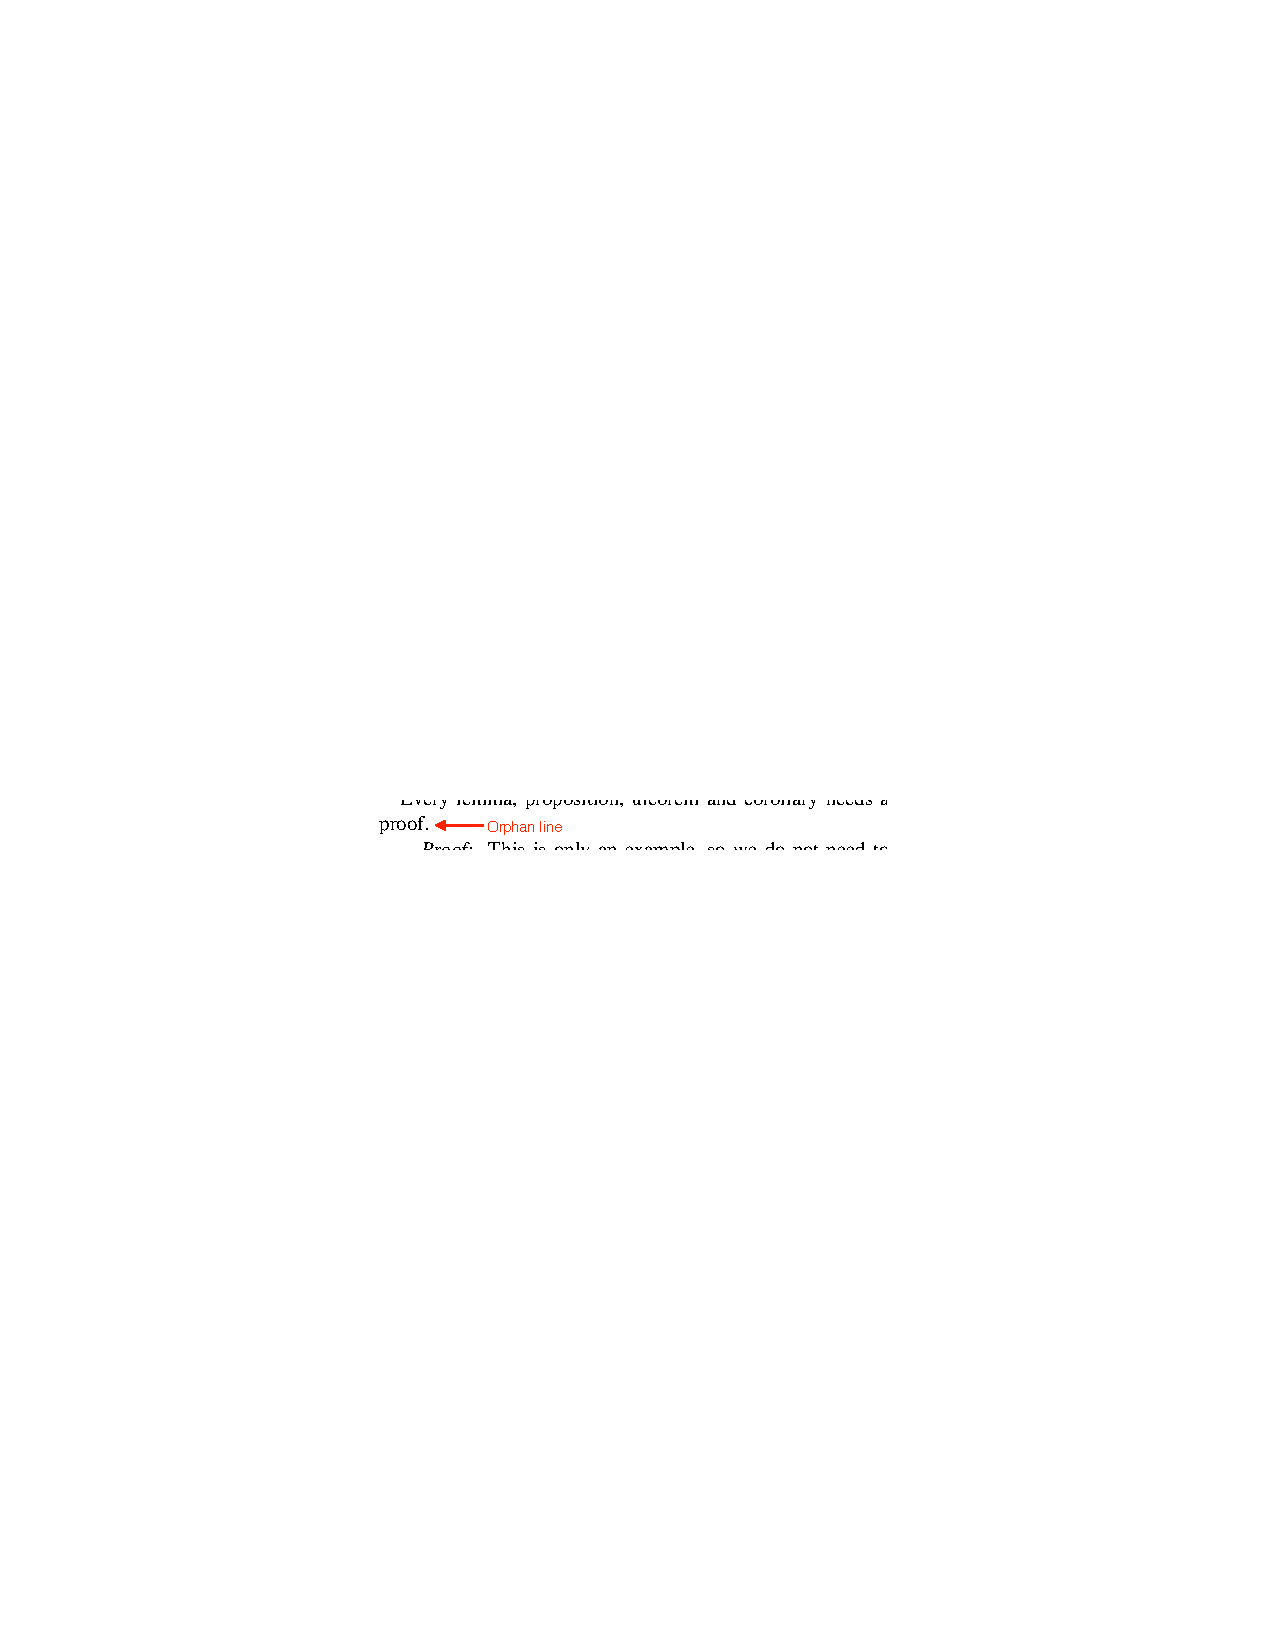
\includegraphics[width=0.9\linewidth]{figures/orphan-line}
  \caption{An example of an orphan line}
  \label{fig:orphan-line}
\end{figure}

\section{TYPESETTING AND ORGANIZATION OF MATHEMATICS}
\subsection{Equations}

Use the AMS Math environments to typeset display-style equations, as the equation below:
\begin{equation}
  \label{eq:newtown-law}
  F=ma.
\end{equation}

Do not use the bare \TeX{} syntax with the double-dollar signs. In general, number all equations (this is the default behavior of the standard equation environments). Punctuate equations with commas or periods when they are part of a sentence. For instance, Euler's law for rotational motion in 2-D is
\begin{equation}
  \label{eq:euler-law}
  \tau=I\alpha,
\end{equation}
where $\tau$ is the sum of torques, $I$ is the moment of inertia, and $\alpha$ is the angular acceleration. The idea is the reader should be able to \emph{read} the equation aloud as text. See also \eqref{eq:newtown-law}.

Be sure that the symbols in your equation have been defined before or immediately following the equation. Refer to equations using the command \texttt{eqref} instead of \texttt{ref} (this will automatically add the parentheses); at the beginning of a sentence, use the word \emph{Equation} as in the following. Equation \eqref{eq:euler-law} is Euler's law of motion.

Get familiar with the \verb|amsmath| package environments for equations (\verb|align|,\verb|gather|,\verb|multline|,\verb|split|), and matrix envinroments with paretheses (\verb|bmatrix|, \verb|Bmatrix|, \verb|vmatrix| and \verb|Vmatrix|).

See the following for a quick reference of most common situations.
\begin{itemize}
\item Aligned equations:
  \begin{align}
      F&=ma,\\
      \tau&=I\alpha.
  \end{align}
  Again, note the use of commas and periods. The same environment can be used to put equations side-by-side:
  \begin{align}
    F&=ma, & \tau&=I\alpha.
  \end{align}
\item Long equations:
  \begin{multline}
    2g(\nabla_XY,Z)=Xg(Y,Z)+Yg(Z,X)-Zg(X,Y)\\
    +g(Z,[X,Y])+g(Y,[Z,X])+g(X,[Z,Y]).
  \end{multline}
  Equations should preferably be broken at equal signs, and plus or minus signs as second option.

\item Matrices and vectors:
  \begin{equation}
    \bmat{
      a_1b_1 & a_1b_2 & \cdots &a_1 b_m\\
      a_2b_1 & \ddots && \vdots\\
      \vdots\\
      a_nb_1&\cdots&&a_nb_m
    }=\bmat{a_1\\\vdots\\a_n}\bmat{b_1 & \cdots & b_m}.
  \end{equation}
\item Optimization problems, sub-equations:
  \begin{subequations}
    \label{eq:sample-optimization}
    \begin{align}
      \min_{Z}\; & \frac{1}{2}\norm{Z-X}^2\label{eq:objective}\\
      \subjectto &   \vct{1}\transpose Z=0,\label{eq:zero-mean-constraint}\\
                 & [X]_1=0.
    \end{align}
  \end{subequations}
  You can then refer to the entire set \eqref{eq:sample-optimization}, or individual sub-equations, such as the objective \eqref{eq:objective} or a specific constraint \eqref{eq:zero-mean-constraint}.
  You can also nest the \var{aligned} enviroment for more complicated constraints:
  \begin{equation}
    \label{eq:sample-optimization-complex}
    \begin{aligned}
      \min_{x,s}\; & s\\
      \subjectto & \left[
                   \begin{aligned}
                           \max_y &x\transpose y\\
                           \subjectto & Ay\leq b
                         \end{aligned}
                   \right]<s\\
                 & \vct{1}\transpose x=1.
    \end{aligned}
  \end{equation}

\item Cases:
  \begin{equation}\label{eq:sign-def}
    \sign(x)=
    \begin{cases}
      1 & \textrm{if } x>0,\\
      -1 & \textrm{if } x<0,\\
      0 & \textrm{otherwise}.
    \end{cases}
  \end{equation}
\end{itemize}

\subsection{Assumptions, Lemmata, Propositions, Theorems}
You can make \emph{blanket assumptions} directly in the text (e.g., ``From now on, we assume that every graph is undirected''). If you need to assume that something holds w.l.o.g., say why; e.g., ``Without loss of generality, we assume that quantities are expressed in meters (we can use other units by multiplying both sides of all equations by the proper conversion factor)''.
If you need to refer back to specific assumptions (e.g., because you are discarding them later in the paper), highlight them with the corresponding environments:
\begin{assumption}\label{assumption:example}
  Every student in this class is assumed to be proficient in the English language.
\end{assumption}
You can then refer back to it as Assumption~\ref{assumption:example}.
If you have three or more assumptions, consider using a labeled enumeration instead. For instance, every student in this class is assumed to:

\begin{lenumerate}{A}
\item \label{it:assumption-english} Be proficient in the English language.
\item Have experience with programming.
\item \label{it:assumption-probability} Have taken a class in probability.
\end{lenumerate}
You can then refer to them as Assumptions~\ref{it:assumption-english}--\ref{it:assumption-probability}.

Definitions are used to establish the meaning of technical terms. You can include multiple related terms in the same definition. The terms that is being defined should be enclosed in the \verb|\emph| macro.
\begin{definition}
  We say that a number is \emph{negative} if it is less than zero, and \emph{non-positive} if it is negative or zero.
\end{definition}

A lemma (lemmata in the plural) is a result (typically, but not always, simple to prove) that is then used as part of a theorem.
\begin{lemma}
  This claim will be used in a theorem.
\end{lemma}

Theorems highlight the most important theoretical results in a paper. You should have only one, and in some rare cases two, main theorems for each paper (not counting preliminary theorems that you might need to quote in the introduction of your paper, see also below).
\begin{theorem}\label{thm:example}
  This claim is the most important of the paper.
\end{theorem}
If you think it is necessary to quote or paraphrase a theorem from another source, or include the common name of a theorem, use the optional argument of the environment.
\begin{theorem}[Localizability \cite{Tron:CDC09}]
  Restate the previous result here.
\end{theorem}


Propositions are lesser results that can stand on their own but are not important as a theorem in the scheme of the paper or are then used in the proof of a theorem.
\begin{proposition}
  An important result, but not as important as a theorem.
\end{proposition}

Corollaries are results (typically with a short proof) that are consequences of a theorem.
\begin{corollary}
  A typical example is the application of Theorem~\ref{thm:example} to a particular, but important, case.
\end{corollary}

Every lemma, proposition, theorem and corollary needs a proof.

\begin{proof}
  This is only an example, so we do not need to actually demonstrate a claim.
\end{proof}
Proofs that are long and from which the reader would not learn anything strictly necessary to understand the paper, can be moved to an appendix; in this case, however, you should still include in the main text an \emph{informal} short statement describing the overall architecture or approach of the proof.

Remarks are used by authors to point out interesting consequences of lemmata, propositions, theorems or proofs. If you need to refer back to a remark, you can include it in an environment.

\begin{remark}
  For remarks to the results of theorems, consider if instead a corollary would be more appropriate.
\end{remark}

\subsection{Various Symbols and Commands}
This section recommendations for miscellaneous mathematical typesetting choices.
\begin{itemize}
\item Use the commands \texttt{norm} and \texttt{abs} for, respectively, $\norm{\cdot}$ and $\abs{\cdot}$.
\item Most of the times, capital letters $A,B,C,\ldots$ are used for matrices; lowercase letters $f,g,v,w,u,s,x,y,\ldots$ are used for vectors, scalars, and functions; calligraphic letters $\cS,\cC$ are used for sets; these, however, are only general guidelines: consistency with previous conventions and uses should take precedence (e.g., see \ref{eq:newtown-law}). The use of the vector accent (e.g., $\vec{v}$) is currently out of fashion.
\item If you want to be really precise, use $(a,b,\ldots)$ for ordered sets (e.g., coordinates, directed edges in graphs) and $\{a,b,\ldots\}$ for unordered sets (undirected edges in graphs).
\item For variables that cycle through different numbers, use the in-set notation, not the equal sign: e.g., $i\in{1,2,\ldots}$ instead of $i=1,2,3$. A variable cannot be equal to multiple different values at the same time.
\item Make sure to define the field and dimensions of vectors and variables, e.g. $v\in\real{d}$, $A\in\complex{d_1\times d_2}$, $s\in\real{}$, and the domain and co-domain for functions and maps, e.g. $f:\real{}\to\real{}$.
\item Most common functions have a corresponding command that will typeset its name correctly: $\exp$, $\log$, $\min$, $\max$, $\argmin$, $\argmax$, $\trace$, $\sin$, $\cos$, $\tan$, $\sign$.
\item If you need to add short text in an equation, use the $\verb|\textrm|$ macro (see \eqref{eq:sign-def} for an example).
\item If you include a number in text that should be treated as an actual mathematical quantity (as opposed to, say, a page number), enclose it in dollar signs to obtain a consistent use of fonts; i.e., use $1234567890$ instead of 1234567890 (notice the difference in the shape of each digit).
\end{itemize}



\subsection{Units}\label{sec:units}
See the following advice when working with units in your writing.
\begin{itemize}
\item Use the \texttt{unit} package to help with the formatting of
  numbers with units. Example: \verb|\unit[25]{\frac{m}{s^2}}}| becomes $\unit[25]{\frac{m}{s^2}}$.
\item Use either SI (MKS) or CGS as primary units. (SI units are encouraged.) English units may be used as secondary units (in parentheses). An exception would be the use of English units as identifiers in trade, such as ``3.5-inch disk drive''.
\item Avoid combining SI and CGS units, such as current in amperes and magnetic field in oersteds. This often leads to confusion because equations do not balance dimensionally. If you must use mixed units, clearly state the units for each quantity that you use in an equation.
\item Do not mix complete spellings and abbreviations of units: $\unit{\frac{Wb}{m^2}}$'' or ``webers per square meter''. Spell out units when they appear in text: ``. . . a few henries'', not ``. . . a few $\unit{H}$''.
\item Use a zero before decimal points: ``$0.25$'', not ``$.25$''. Use
  ``$\unit{cm^3}$'', not ``$\unit{cc}$''.)
\end{itemize}



\section{FIGURES, TABLES, AND ALGORITHMS}
Place figures, tables, and algorithms at the top and bottom of columns. Avoid placing them in the middle of columns. Large figures, tables, and algorithms may span across both columns. Figure captions should be below the figures; table heads should appear above the tables (this will be handled automatically by the \verb|\caption| command). Insert figures and tables around where they are cited in the text (never on a previous page). To center the content, use the command \verb|\centering| (the enviroment \verb|center| achieves a similar result but adds vertical spaces that are typically unwanted).

\subsection{Figures}

Use the abbreviation Fig.~\ref{fig:trajectories}, even at the beginning of a sentence.

\begin{table}[t]
\caption{An Example of a Table}
\label{table:example}
\centering
\begin{tabular}{lllll}
  \toprule
  &\multicolumn{2}{c}{Group A}
  &\multicolumn{2}{c}{Group B} \\
  \cmidrule(lr){2-3} \cmidrule(l){4-5}
  &Age
  &Height
  &Grade
  &Perc.\\
  \midrule
  First year & 4 & 8 & 4 & 18 \\
  Second year & 4 & 8 & 4 & 18 \\
  \bottomrule
\end{tabular}
\end{table}

Make sure the text in the figure is of a size consistent with the surrounding text (e.g., axes labels of the same size as the caption, e.g., see Fig.~\ref{fig:trajectories}), and that the formatting of the figures is consistent across all figures. The easiest way to enforce this is to output the original figure (e.g., from Matlab) directly to the right size (i.e., you should not need to use \verb|width|,  \verb|height| or \verb|scale| arguments to the \verb|includegraphics| command) and adjust the font sizes in the original graph (i.e., in Matlab). Do not include the extension in the filename given to the \verb|includegraphics| command  ({\LaTeX} will automatically look for all suitable extensions). Always use a vectorial graphic format (typically PDF, as they allow unlimited zoom without quality loss, compare Fig.~\ref{fig:trajectories-base} and Fig.~\ref{fig:trajectories-base-rasterized}), except for real pictures (e.g., a photo of an experiment). Files in the EPS format can be easily converted to PDF using the \verb|epspdf| or \verb|epstopdf| commands in a terminal. Preferably, all graphics files should be in a \verb|figures| subfolder. Avoid 3-D plots (they are typically harder to read than a 2-D equivalent, and transparency, in Matlab, does not vectorize well), unless you have a very good reason, and also a second good reason for the first good reason.
Use the command \verb|subfloat| to create subfigures. Use double-line-breaks in the source file to control which figures are side-by-side, and which are one on top of the other (as in standard text). Unless you are short on space, always labels also for subfigures (even if you do not have a caption), so that you can always refer to them, as for Fig.~\ref{fig:trajectories-base}. If possible, use the same name for the file and the \LaTeX{} label.
\begin{figure*}[t]
  \centering
  \subfloat[High quality, vectorial version]{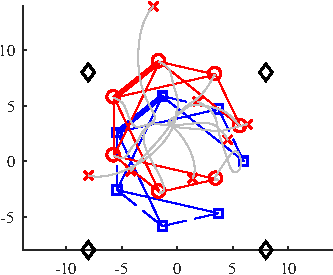
\includegraphics{figures/trajectories-base}\label{fig:trajectories-base}}% note the double line break below causes the figure to be formatted below the other
  \subfloat[Lower quality, rasterized version]{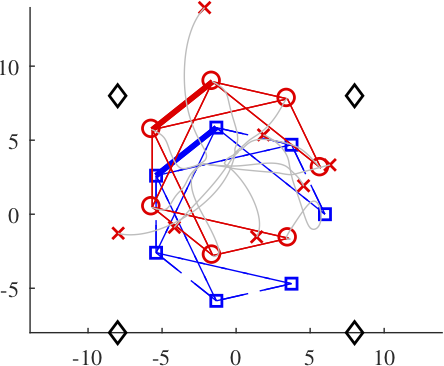
\includegraphics{figures/trajectories-base-raster}\label{fig:trajectories-base-rasterized}}
  \subfloat[Another figure]{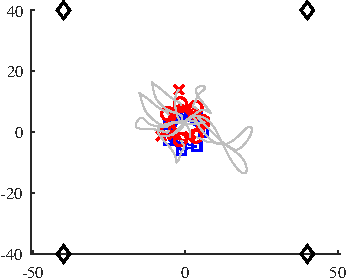
\includegraphics{figures/trajectories-scaled}\label{fig:trajectories-scaled}}
  \caption{An example of a figure with multiple subfigures. You can refer to subfigures in the main caption, as shown in the next sentence, but you need to protect the command (see source). To see the difference between \protect\subref{fig:trajectories-base} and \protect\subref{fig:trajectories-base-rasterized}, use the maximum zoom level on your PDF viewer}
  \label{fig:trajectories}
\end{figure*}

\subsection{Tables}
 Use the \texttt{booktabs} package to format tables in a professional, uncluttered way, e.g., see Table~\ref{table:example} \rtron{Add bibref to booktabs docs}. Absolutely avoid using double lines to separate lines or columns.

\subsection{Algorithms}
For algorithms, use the \verb|algorithm| environment for the float, and the \verb|algorithmic| environment for the actual algorithm (these are conceptually similar to \verb|table| and \verb|tabular|). See Algorithm~\ref{algo:gradient} for an example. You can refer to specific lines in the algorithm: e.g., line \ref{it:gradient} contains the main update step of the algorithm.

\begin{algorithm}
  \begin{algorithmic}[1]
    \Require The gradient $\nabla f$ of a function $f:\real{}\to\real{}$, number of iterations $N$, a step size $\varepsilon$.
    \Ensure A local optimizer $x^\ast\in\real{}$.
    \State Let $x\gets 0$ \Comment{This is a comment}
    \For{$k\in{1,\ldots,N}$}

    \State $x\gets x-\varepsilon\nabla f(x)$. \label{it:gradient}
    \EndFor
    \State Let $x^\ast\gets x$
    \label{it:endwhile}
  \end{algorithmic}
  \caption{Simplest version of gradient descent.}
  \label{algo:gradient}
\end{algorithm}

 %%%%%%%%%%%%%%%%%%%%
 \addtolength{\textheight}{-7.2cm}   % This command serves to balance the column lengths
 % on the last page of the document manually. It shortens
 % the textheight of the last page by a suitable amount.
 % This command does not take effect until the next page
 % so it should come on the page before the last. Make
 % sure that you do not shorten the textheight too much.
 %%%%%%%%%%%%%%%%%%%%

\section{IN-LINE COMMENTING FACILITIES}
This template includes commands for inserting in-line comments in the text. First, you need to define a new \emph{commenter} with the command \verb|\newcommenter{name}{colorName}|, where \verb|name| is the commenter's name, and \verb|colorName| is the name of a color (please refer to the documentation of the \var{xcolor} package for a list of valid names). For instance, the preamble of this template creates the commenter \var{todo}. You can then insert comments using \verb|\todo{Text of the comment}|, and you can mention a commenter names using the command \verb|\atname|, substituting \verb|name| with the commenter's name. \todo{This is an example of a comment, with a mention of the same commenter: \attodo.}

\section{\LaTeX{} CODING CONVENTIONS}
\subsection{Internal cross references}
\label{sec:internal-xrefs}
You can assign a label to various objects in the documents, and then use this label to
Labels can be defined with the following command \verb|\label{abbreviation:name}|. The first part, \verb|abbreviation:|, should be \verb|eq:| for equations, \verb|tab:| for tables, \verb|fig:| for figures, \verb|it:| for items in a list, and \verb|sec:| for sections. The second part should be a descriptive but short name for the referred object (e.g., do not use numbers). Note that, for figures, it is generally safer to place the \var{label} command after the caption (otherwise, in some cases the label will refer to the previous paragraph).
You can refer back to a label with the command \verb|\ref{abbreviation:name}|. To avoid a line break just before a reference number, use a non-breaking space as follows (see the source code), Section~\ref{sec:internal-xrefs}; an exception is typically made for for equations, for which you should use \verb|\eqref| (this command automatically includes parentheses around the equation number).

\section{CONCLUSIONS}

A conclusion section is not required. Although a conclusion may review the main points of the paper, do not replicate the abstract as the conclusion. A conclusion typically elaborates on the importance of the work and suggests future applications and extensions.


\section*{APPENDIX}

Appendixes should appear before the acknowledgment.

\section*{ACKNOWLEDGMENT}

The preferred spelling of the word acknowledgment in America is without an e after the g. Avoid the stilted expression, One of us (R. B. G.) thanks . . .  Instead, try R. B. G. thanks. Put sponsor acknowledgments in the unnumbered footnote on the first page.

\section*{REFERENCES}
References are important to the reader; therefore, each citation must be complete and correct. If at all possible, references should be commonly available publications. Use BibTeX and \texttt{.bib} files for organizing your bibliography. Put all your files under the \texttt{biblio} subdirectory. Note that a reference is listed at the end of the paper only if it is actually cited. You can group multiple references in the same citation commands (these will probably be automatically \emph{compressed} to save space). For instance, only these papers will be cited \cite{Tron:CVPR07,Tron:CDC09,Tron:SPM11,nestmeyer2015decentralized}. In the IEEE style, citations appear as part of the sentence, not after the period. You can also refer to specific Theorems, Propositions and similar, as in \cite[Prop. 1]{Tron:CDC09}. In your \texttt{bib} files, use BibTeX strings for the name of conferences and journals; in this way you will ensure that different items have a consistent naming (e.g., with the use of abbreviations). See the files \texttt{biblio/IEEEfull}, \texttt{biblio/IEEEConfFull}, and \texttt{biblio/OtherFull} for examples of string definitions.
\todo{Add examples.}

\bibliographystyle{biblio/ieee}

\bibliography{biblio/IEEEfull,biblio/IEEEConfFull,biblio/OtherFull,% Do not insert spaces in this command, otherwise it will not work.
  biblio/tron,%
  biblio/writing,%
  biblio/formationControl,%
  biblio/websites}


\end{document}
